\documentclass[../main.tex]{subfiles}
\graphicspath{{\subfix{../figures/}}}
\usepackage{amsmath}
\begin{document}

\subsection{Background}
Modern vehicles require multiple redundant and complementary sensors in order to fully provide driver assistance and autonomus driving capabilities. Automotive radar is a prominent sensor for these use-cases due its invariance to weather and lighting, and its long detection range \cite{bilik_radar_2019}.

\par
A common phenomena in radar sensors, and specifically in automotive radar, is the multipath induced ghost targets (see fig. \ref{fig:multipath}). This phenomena occurs in the presence of reflective surfaces from which the radar signal can bounce and reach a single target in multiple paths. The direct signal path induce a real target at the physical target location, and the indirect paths induce ghost targets as reflections of the real target. 

\par
In high-resolution automotive radar, this hinders the probability of detection (PD), but more notably, the probablity of false alarm (PFA). The reflected signals from both the real and ghost targets are processed jointly, thus reducing SNR and PD. As radar resolution increases, the real and ghost targets will be localized to different range-azimuth bins, which greatly increases PFA \cite{bilik_radar_2019}.


\begin{figure}[ht!]
  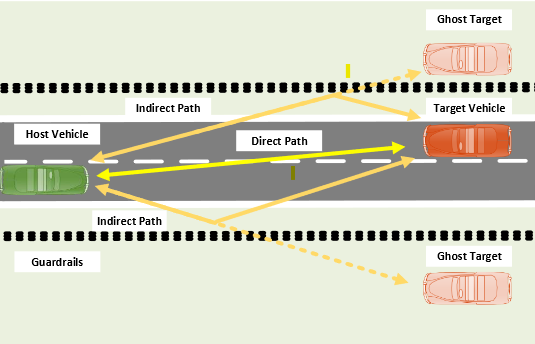
\includegraphics[scale=0.6]{figures/multipath.png}
  \caption{Exemplar automotive environment with reflective surfaces (guardrails and road surface) that induce the multipath phenomena.}
  \label{fig:multipath}
\end{figure}

\subsection{Radar Processing}
Automotive radars are commonly high-resolution linear ferquency modulated continous wave (FMCW). Given a signal with amplitude $A_t$, a carrier ferquency $f_c$, chirp duration $T$ and chirp slope $\alpha$, the radar chirp signal is given by:
\begin{equation}
s_t(t) = A_t e^{-2 \pi j(f_c t+\frac{1}{2}\alpha t^2)}
\end{equation} 


The received signal in the scenario illustrated in fig.\ref*{fig:multipath} includes signal returned from the direct path $s_r$ along with the signal returned from the indirect path $s_g$: 
\begin{align}
s_{tot}(t) = s_r(t) + s_g(t) \\
s_r(t) = A_r e^{-2 \pi j(f_c (t-\tau_r)+\frac{1}{2}\alpha (t-\tau_r)^2)} \\
s_g(t) = A_g e^{-2 \pi j(f_c (t-\tau_g)+\frac{1}{2}\alpha (t-\tau_g)^2)} \\
\end{align} 
where $ \tau _g > \tau_r $ are time delays, $A_r$ and $A_g$ are attenuated amplitudes of the direct and indirect signals.\par

Traditional linear FMCW processing perfoms dechirping by mixing the received signal with the transmitted signal, followed by 3D-FFT to obtain a data cube in range-azimuth-doppler space. the resolution of a single cell is a function of carrier ferquency $f_c$ and chirp bandwidth $B = \alpha T$:
\begin{align}
\triangle R = \frac{c}{2B} \\
\triangle V_{dop} = \frac{c}{2f_c T} \\
\triangle \theta = \theta_B \\
\end{align}


\end{document}